%=================================================================
%\documentclass{article}%[article,accept,moreauthors,pdftex,10pt,a4paper]{Definitions/mdpi}
\documentclass[article,accept,moreauthors,pdftex,10pt,a4paper]{../MDPI_template/Definitions/mdpi}
%\usepackage[lite]{mtpro2}
\usepackage{scalerel}
\firstpage{1} 
\makeatletter 
\setcounter{page}{\@firstpage} 

\Title{Simulation of Positron Shower Leakage}
% Authors, for the paper (add full first names)
%\Author{Nandita Raha, Marco Incagli, Stfeno di Falco \\$~INFN ~Pisa$}

\abstract{
One of the goals of this study is to understand and quantify the leakage of the positron 
showers in the passage through our calorimeters and then add it back to the observed energy. 
This study has been done as a function of the positron energy, impinging point on the calorimeter face, 
angle of incidence, ...  We need to understand how the radiation is lost in the passage through 
$\mathrm{PbF_2}$ crystals. Leakage effects at boundaries between crystals can be larger than when the positron 
hits the center of a crystal. The positrons emanating from muons decaying at the magic momentum 
on the ideal orbit would have a different angular distribution compared to the off-track ones. 
Thus we expect a different rate in the 9$\times$6 grid structure of our calorimeter.  
There could also be other effects due to beam oscillations etc. All this needs to be quantified with simulations. 
The simulations in this note have been done using Geant4.} 
%In the next step, we could study the effect of the spectrum with a 
%varying incident angle of the beam.
%The energy spectrum of the muon losses can also be simulated and investigated for the most simple case i.e. 
%muons of 3.1 GeV shot perpendicular to the crystal. These so-called "lost muon events" have been studied in 
%detail and show a peak energy of 170 MeV , when crossing a single crystal. This would be a good exercise 
%since we have data to verify the simulation.}
\begin{document}

%USE: $\mathrm{formula/equation}$ to remove Italics

\section{Introduction}
The Muon g-2 experiment uses 24 calorimeters surrounding a circular storage ring. Each calorimeter is made up of 
a matrix of 9$\times$6 segmented $\mathrm{PbF_2}$ crystals (2.5$\times$2.5$\times$14 cm$^3$) read by 
Silicon Photo Multipliers (SiPMs). We use $\mathrm{PbF_2}$ crystals since they have a high density 
and high refractive index. 
Its high density allows the containment of the positron shower in a small area  
thereby preventing losses or leakages. The Moliere radius of $\mathrm{PbF_2}$ is 2.1 cm which is greater than 
2.5 cm thereby allowing 90\% of the shower to be contained within the crystals \cite{c1}. 
The high refractive index of $\mathrm{PbF_2}$ produces Cherenkov radiation corresponding to an energy threshold 
of $\approx$ 100 keV for positrons. The energy threshold of positrons for measuring $\omega_a$ is above 1 GeV, which is 
favourable for our experiment. Finally, the light yield of Cherenkov detectors are proportional to incident 
particle energy that will enable an accurate and easy energy calibration. 
In the passage of muons through these detectors, we include all physical processes it undergoes before decaying to 
positrons in our simulation. Some of these processes include Cherenkov radiation, transition radiation, bremsstrahlung 
and pair production \cite{c2}. %All possible orinetations, positions and angles have been studied to check their 
%dependence on the energy. 
The positrons incident at varies positions in a crystal have been studied to check its dependence on the energy.
The leakage of the positron shower with varying energy is also studied here.  

\noindent 
\section{Positrons through Lead--Fluoride Crystals}
A visualization of the simulation of the positron shower using Geant4 for 10000 events 
incident perpendicular on the XY--plane of crystal 22 of the 9$\times$6 segmented $\mathrm{PbF_2}$
 crystals (2.5$\times$2.5$\times$14 cm$^3$) is shown in figure \ref{fig1}.
\begin{figure}[H]
\centering
%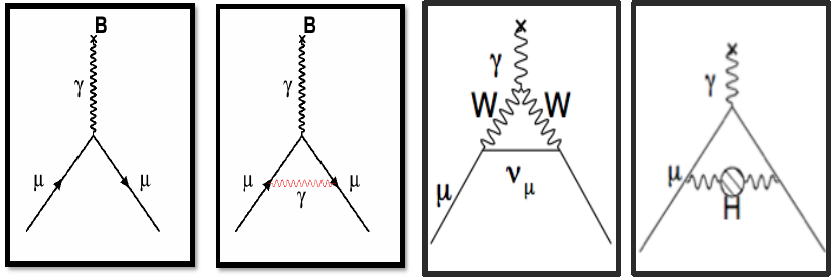
\includegraphics[width=2 cm]{a_mu_corrections.png}
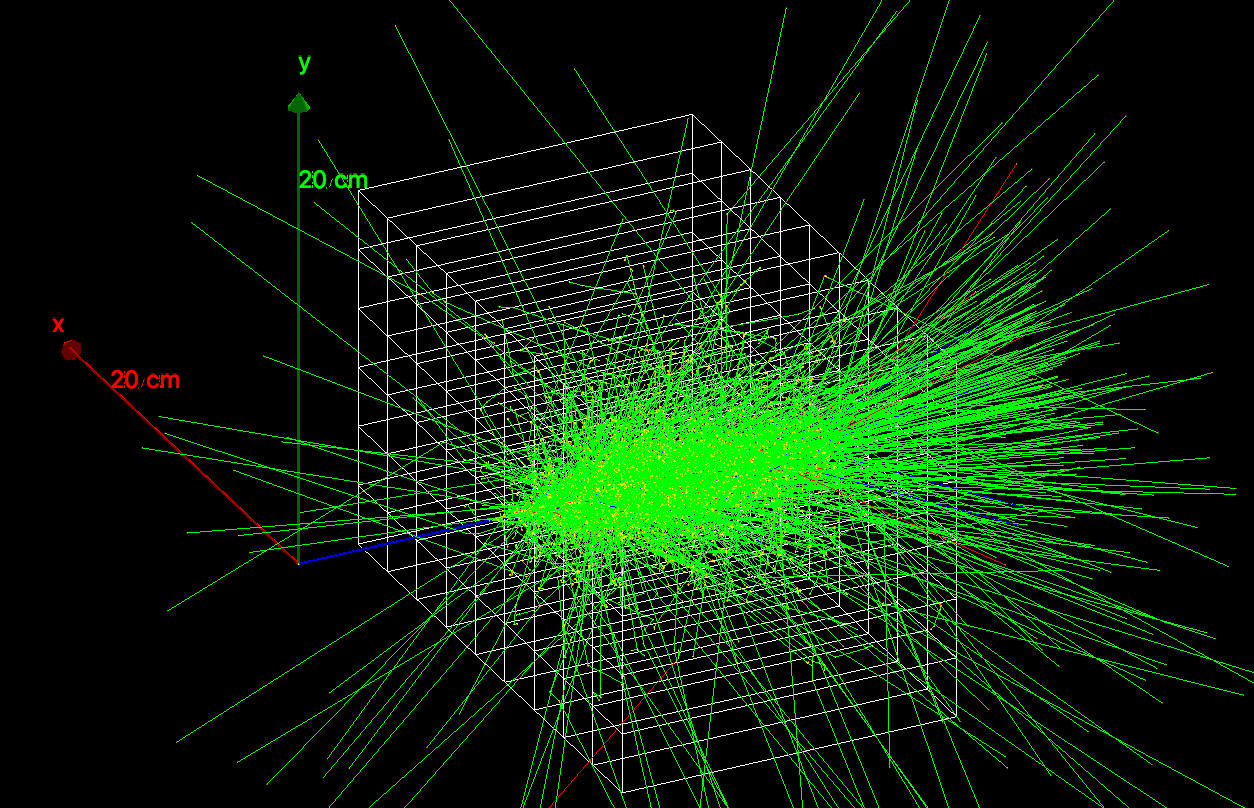
\includegraphics[width=8 cm]{visual.png}
\caption{\label{fig1} Visualization of 10000 events passing through the center of crystal 22. }
\end{figure}
The beam is along the Z-direction with an energy of 3.1 GeV hitting the center of the matrix 
(no lateral leakage). Crystal 22 (counting from zero) was selected since it is almost centrally located. 
 The default color scheme has been used showing the electrons in red, positrons in blue 
and gamma rays in green. The blue line at the origin along the z-axis denotes the original positron beam. 

Figure \ref{fig2} below shows the sum of the energies of all the particles in the positron 
shower that pass through the 9$\times$6 segmented $\mathrm{PbF_2}$ crystals for the above-mentioned configuration. 
Note that the mean energy collected for a positron beam of initial energy 3100 MeV is 2913 MeV which is about 93.9\%, 
indicating a leakage of about 6.1\% of the initial energy of 3.1 GeV.
\begin{figure}[H]
\centering
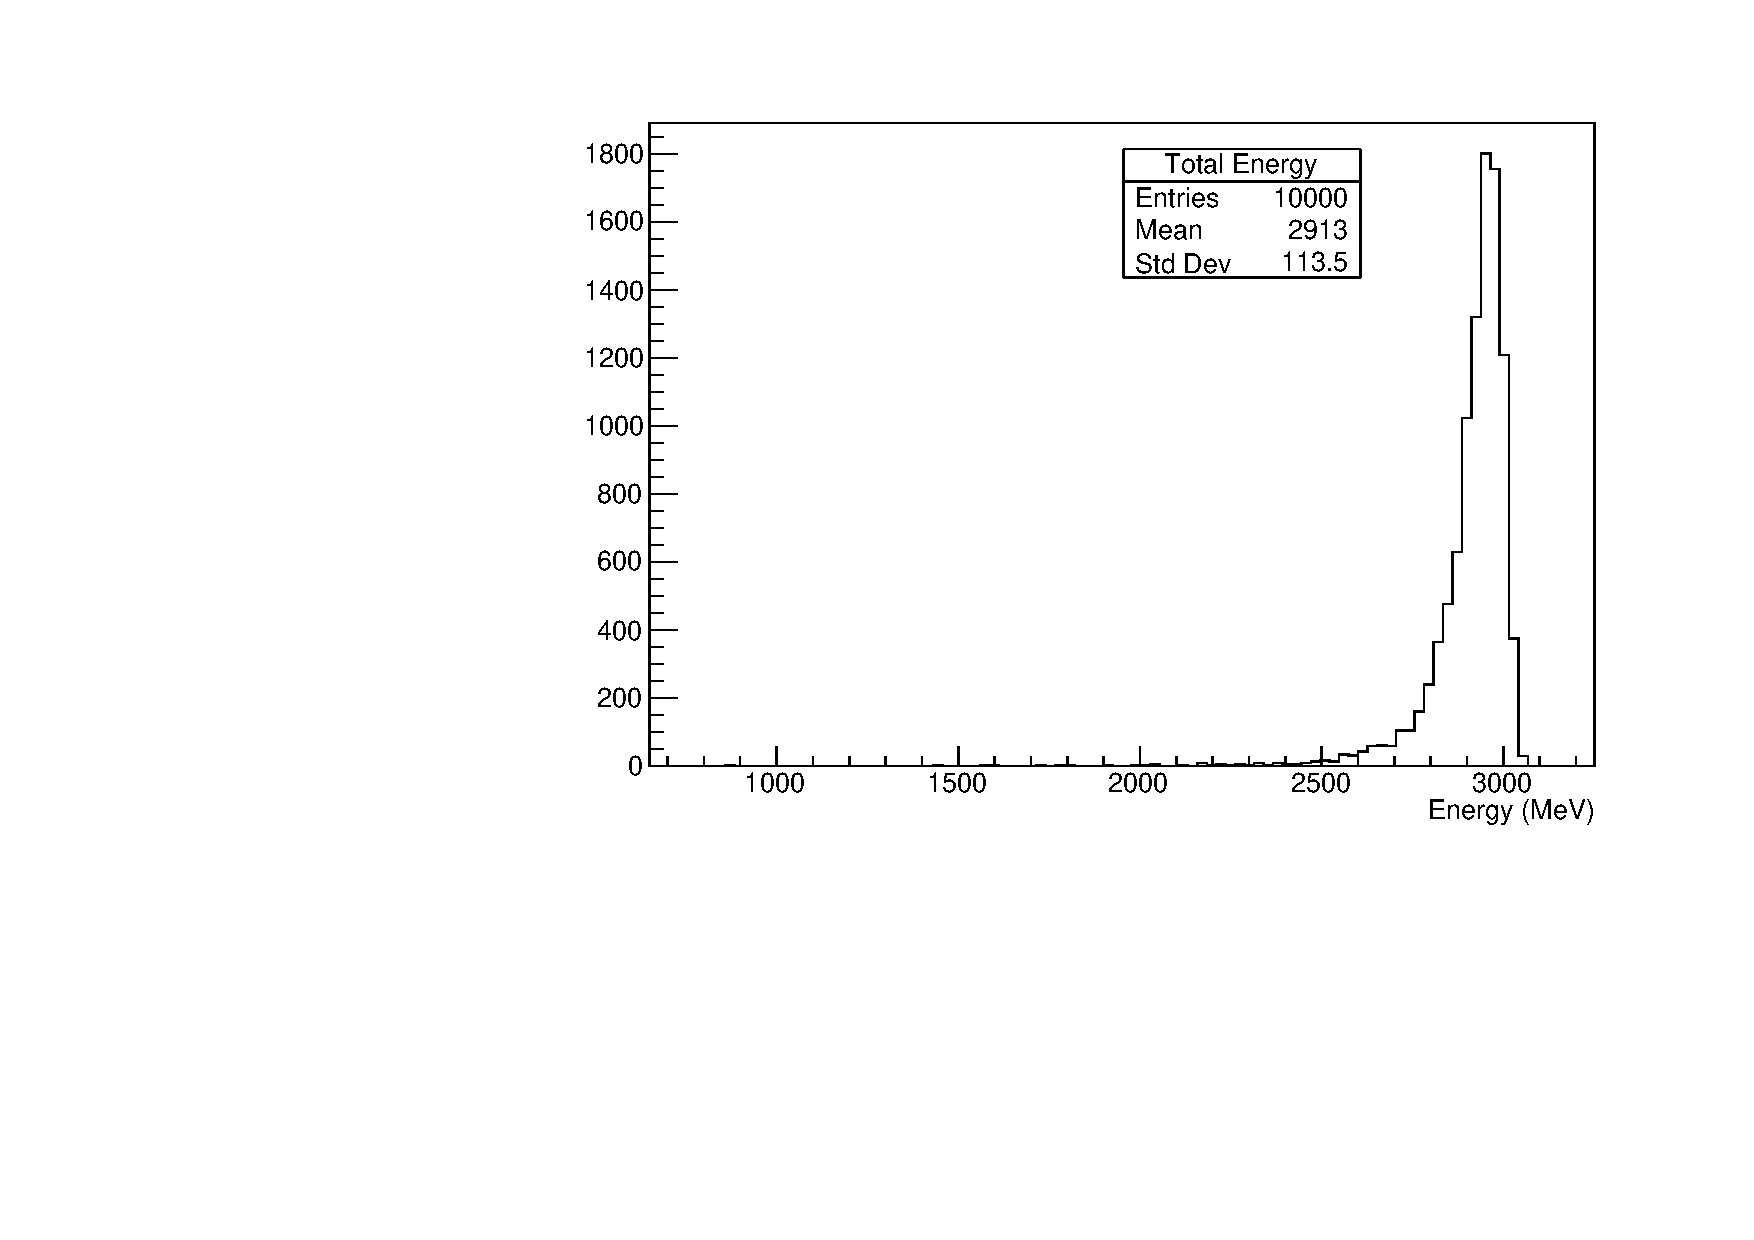
\includegraphics[width=10 cm]{total_energy.pdf}
\caption{\label{fig2}.Total positron energy spectrum of all particles of energy 3.1 GeV.}
\end{figure} 

To check the dependence of the energy distribution on the beam position we considered 
the beam incident normally on at three positions of crystal 22 - center, 
top (1 mm below the upper edge) 
and bottom (1 mm above the lower edge) of this crystal. The energy spectrum of the positron shower through 
the 9$\times$6 grid system of the experimental setup for these three positions is shown in \ref{fig3}. This 
is the sum of energies of all crystals. Note that the distribution about the center is almost symmetrical. 
Thus, the left and right plots of figure \ref{fig3} have a similar distribution. 
%as a sum of energies . 

\begin{figure}[H]
\centering
%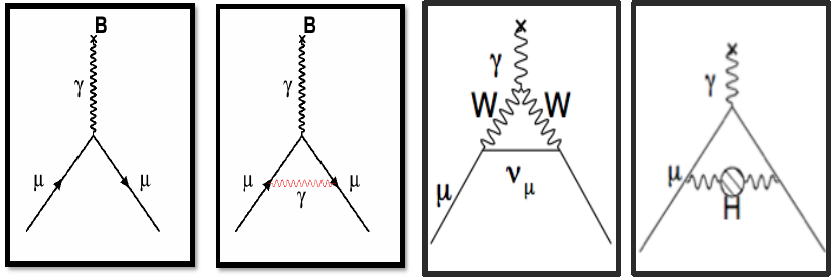
\includegraphics[width=2 cm]{a_mu_corrections.png}
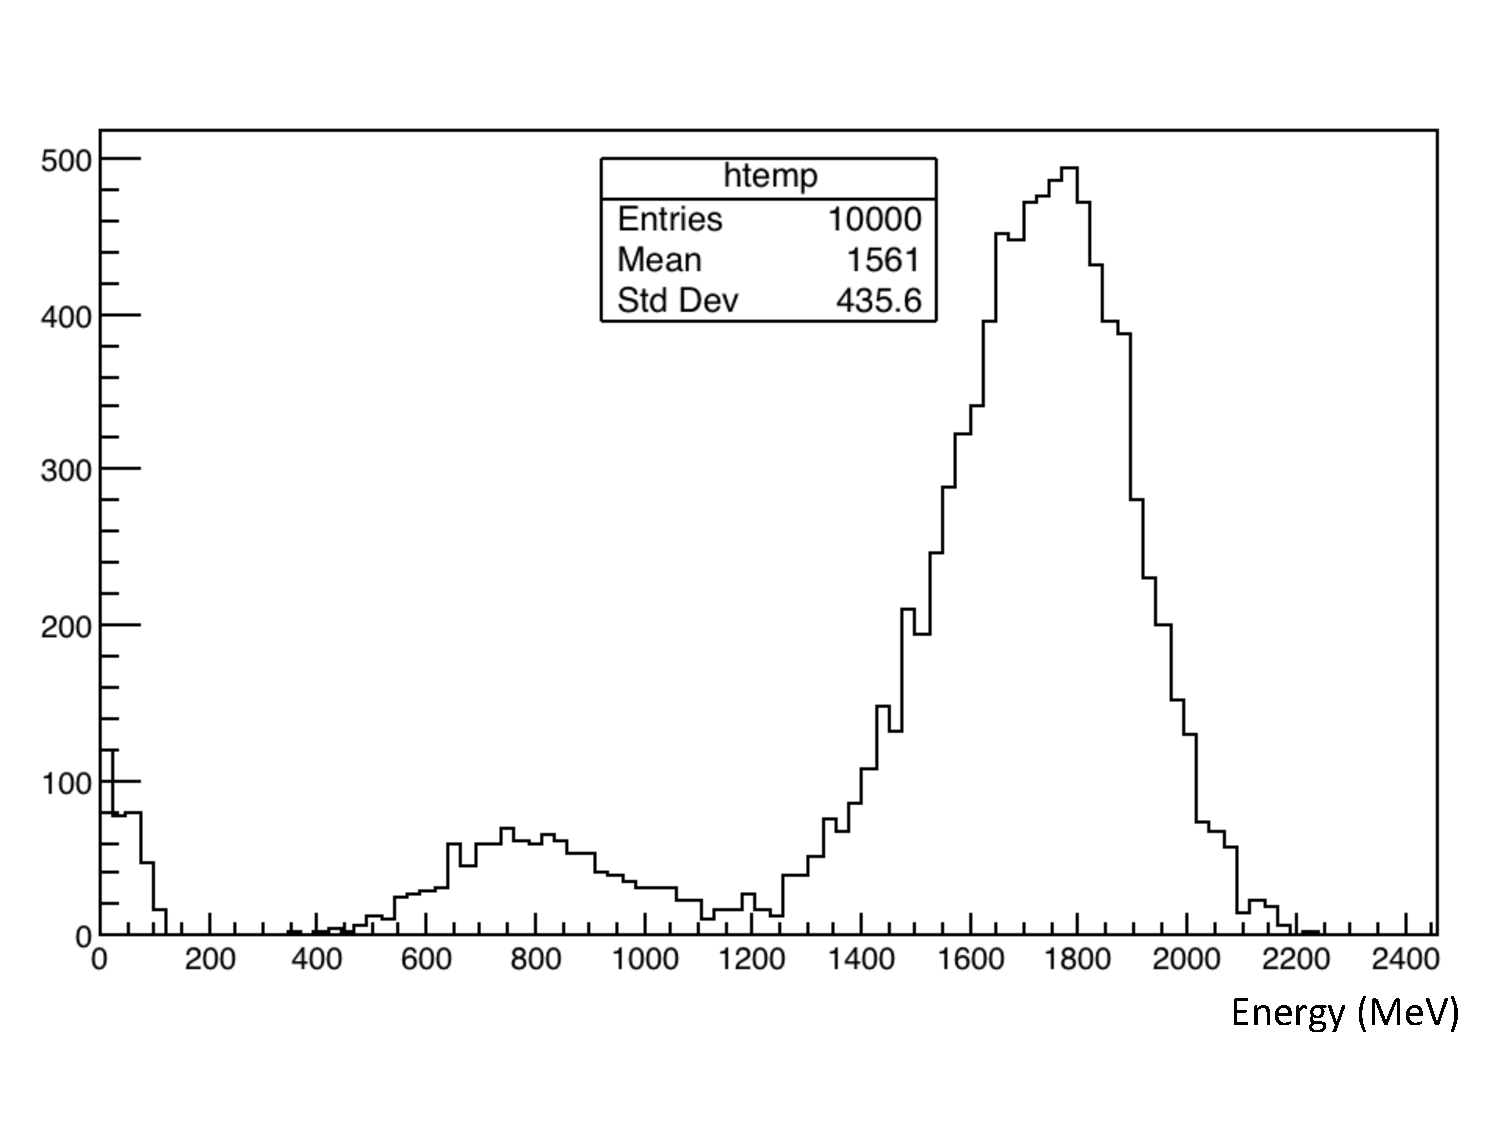
\includegraphics[width=5 cm]{leakage_all_top.pdf}
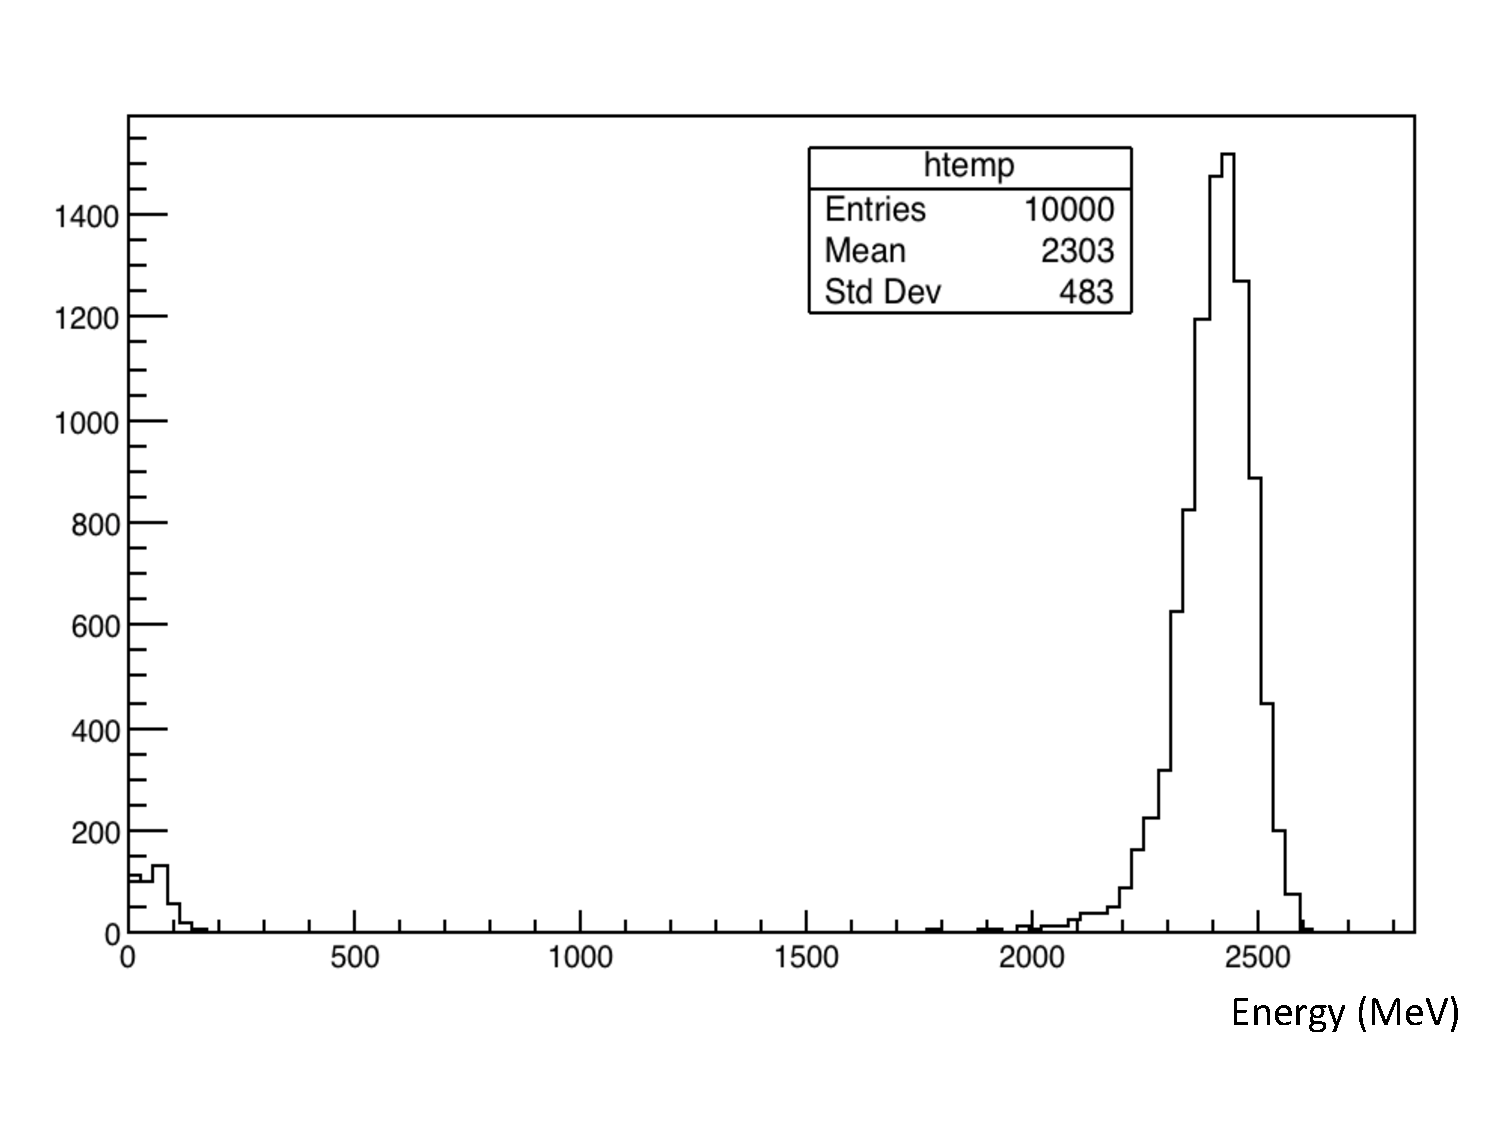
\includegraphics[width=5 cm]{leakage_all_center.pdf}
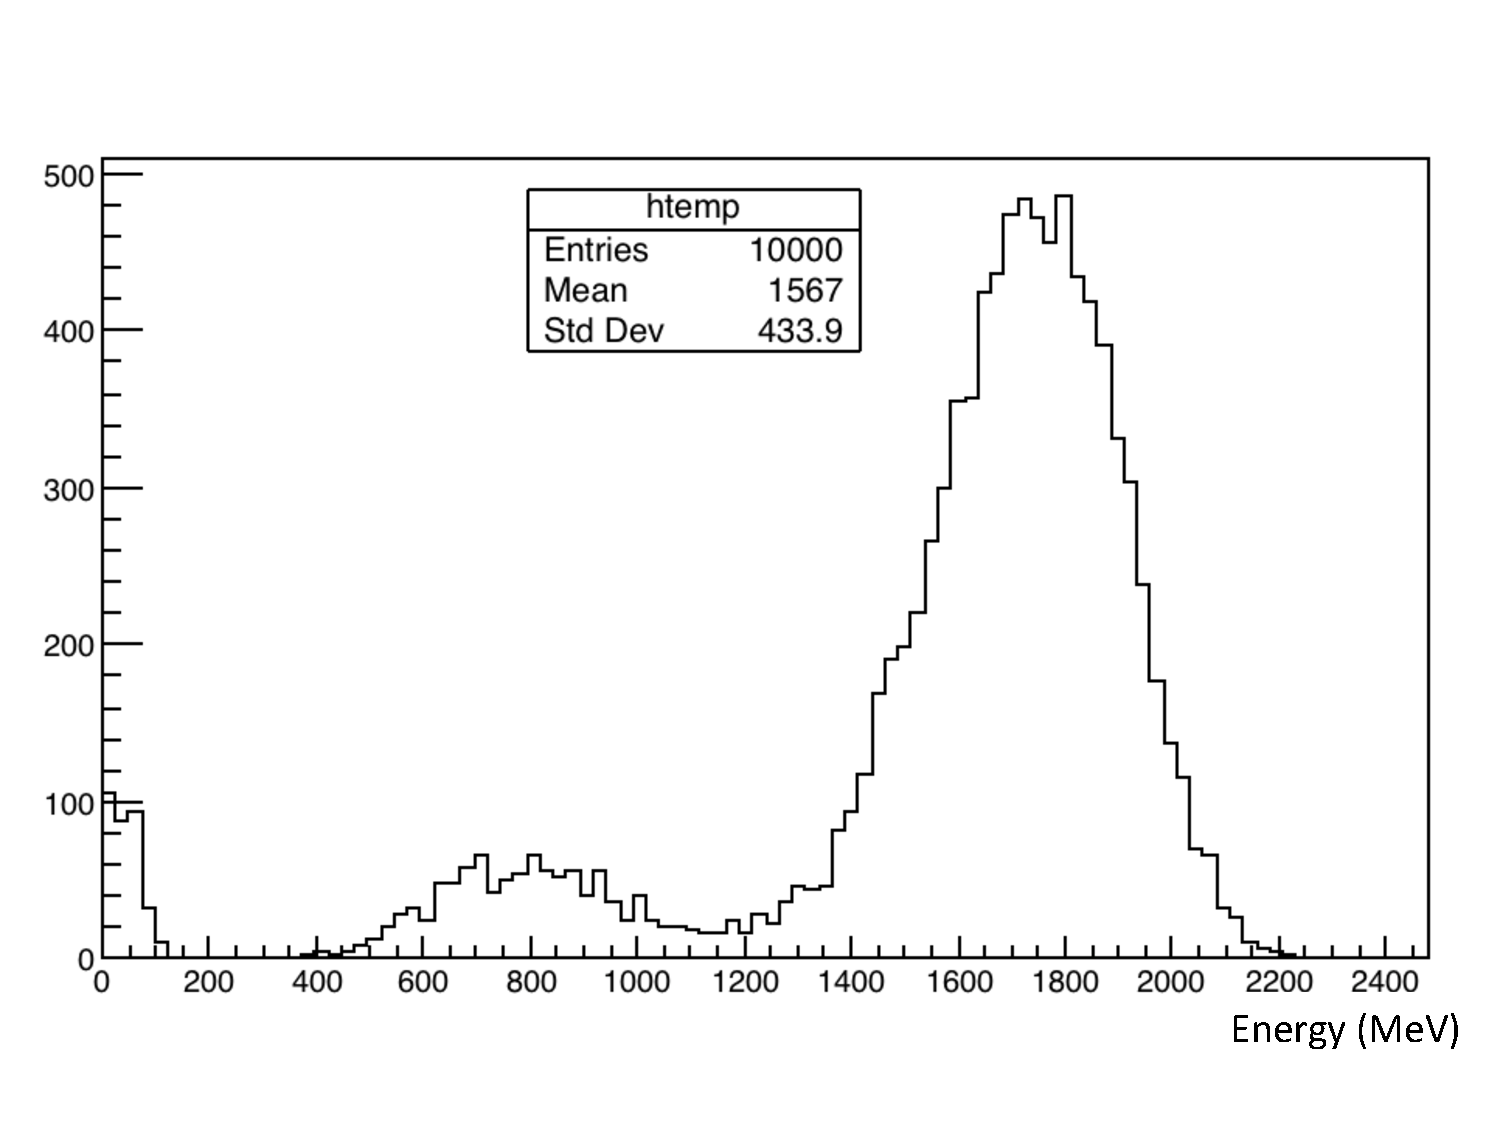
\includegraphics[width=5 cm]{leakage_all_bottom.pdf}
%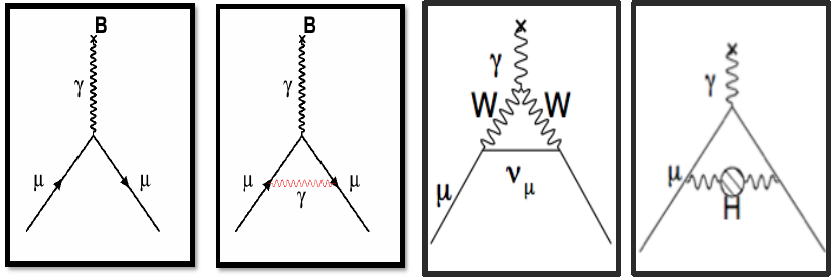
\includegraphics{a_mu_corrections.pdf}
\caption{\label{fig3} The positron energy distribution through a 9$\times$6 segmented $\mathrm{PbF_2}$ crystals of a 
calorimeter when the moun beam is incident at the top (left panel - 9.5 mm above the center) center (middle panel) 
and bottom (right panel - 9.5 mm below the center) of crystal 22 respectively. This depicts the positron shower leakage 
in a calorimeter.}
\end{figure}  

The number of positrons hitting the crystals for these three cases is shown in figure \ref{fig4}. 
We used a log scale to visualize better the distribution in each crystal. Notice the distribution is almost symmetrical 
about crystal 22 when the beam hits the center of crystal 22 (middle panel of figure \ref{fig4}). 
The number of hits are more above crystal 22 when the beam moves above the center (left panel of figure \ref{fig4}). 
Similarly, the number of hits are more below crystal 22 when the beam moves 
below the center (right panel of figure \ref{fig4}) which is obvious. 
\begin{figure}[H]
\centering
%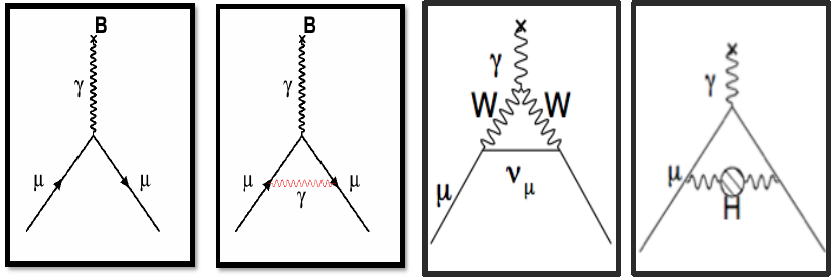
\includegraphics[width=2 cm]{a_mu_corrections.png}
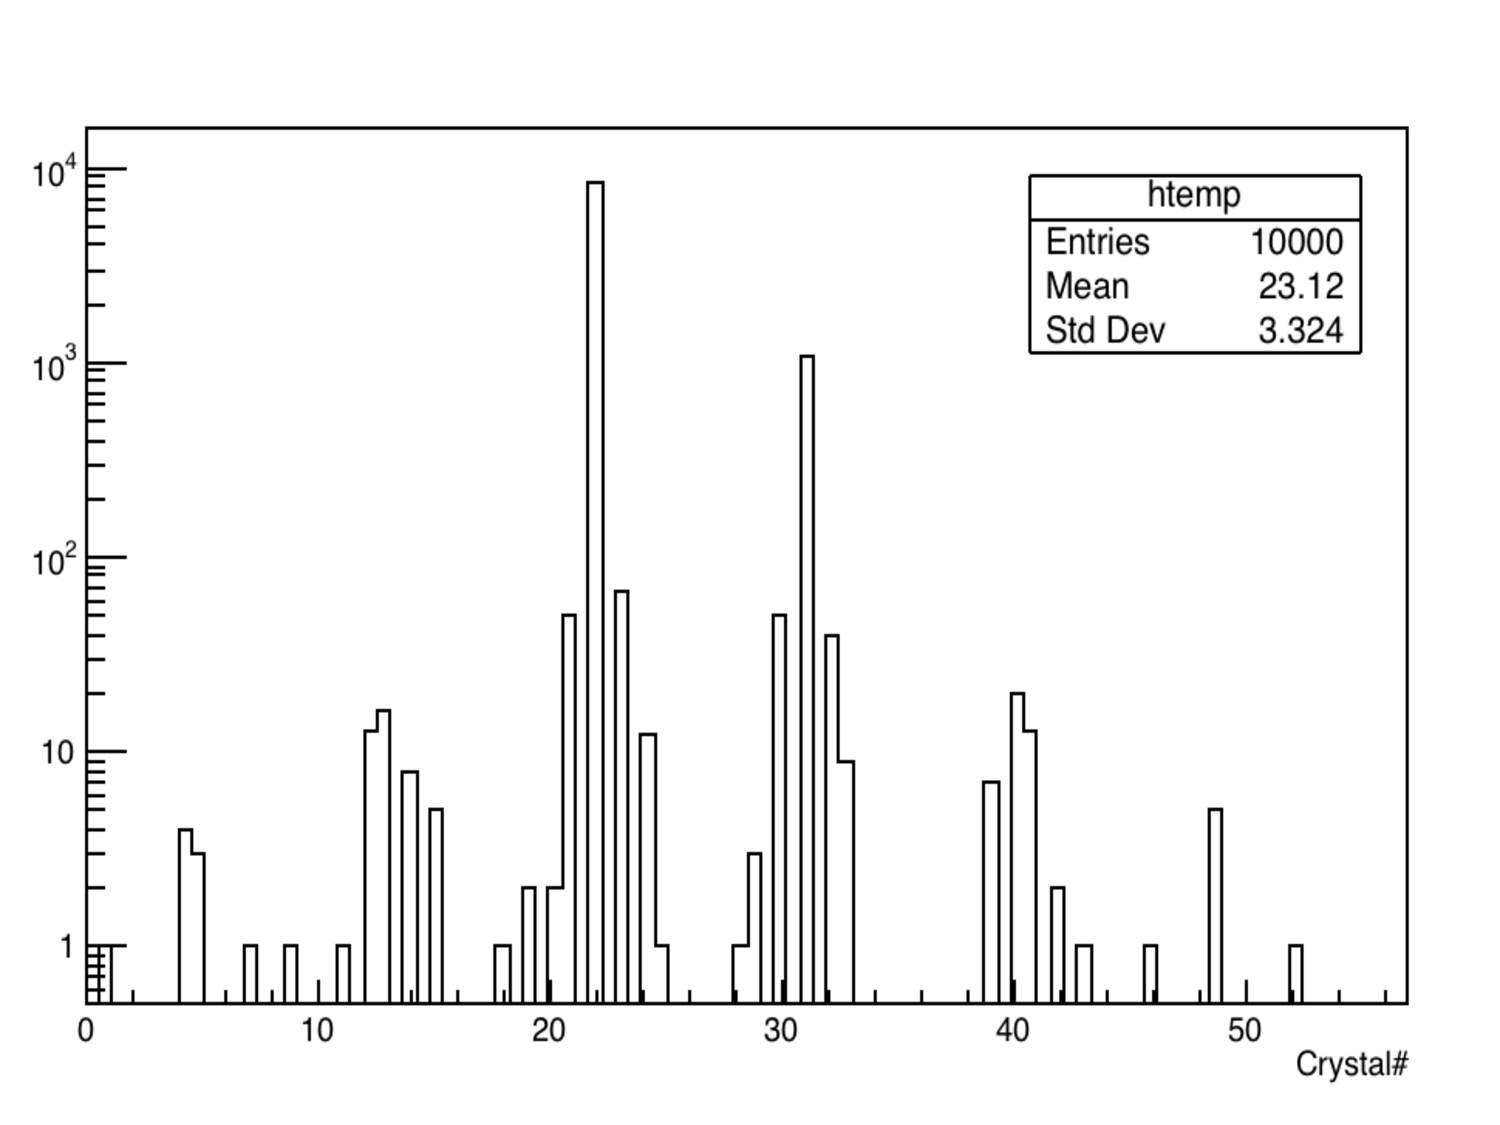
\includegraphics[width=5 cm]{dist_all_top.pdf}
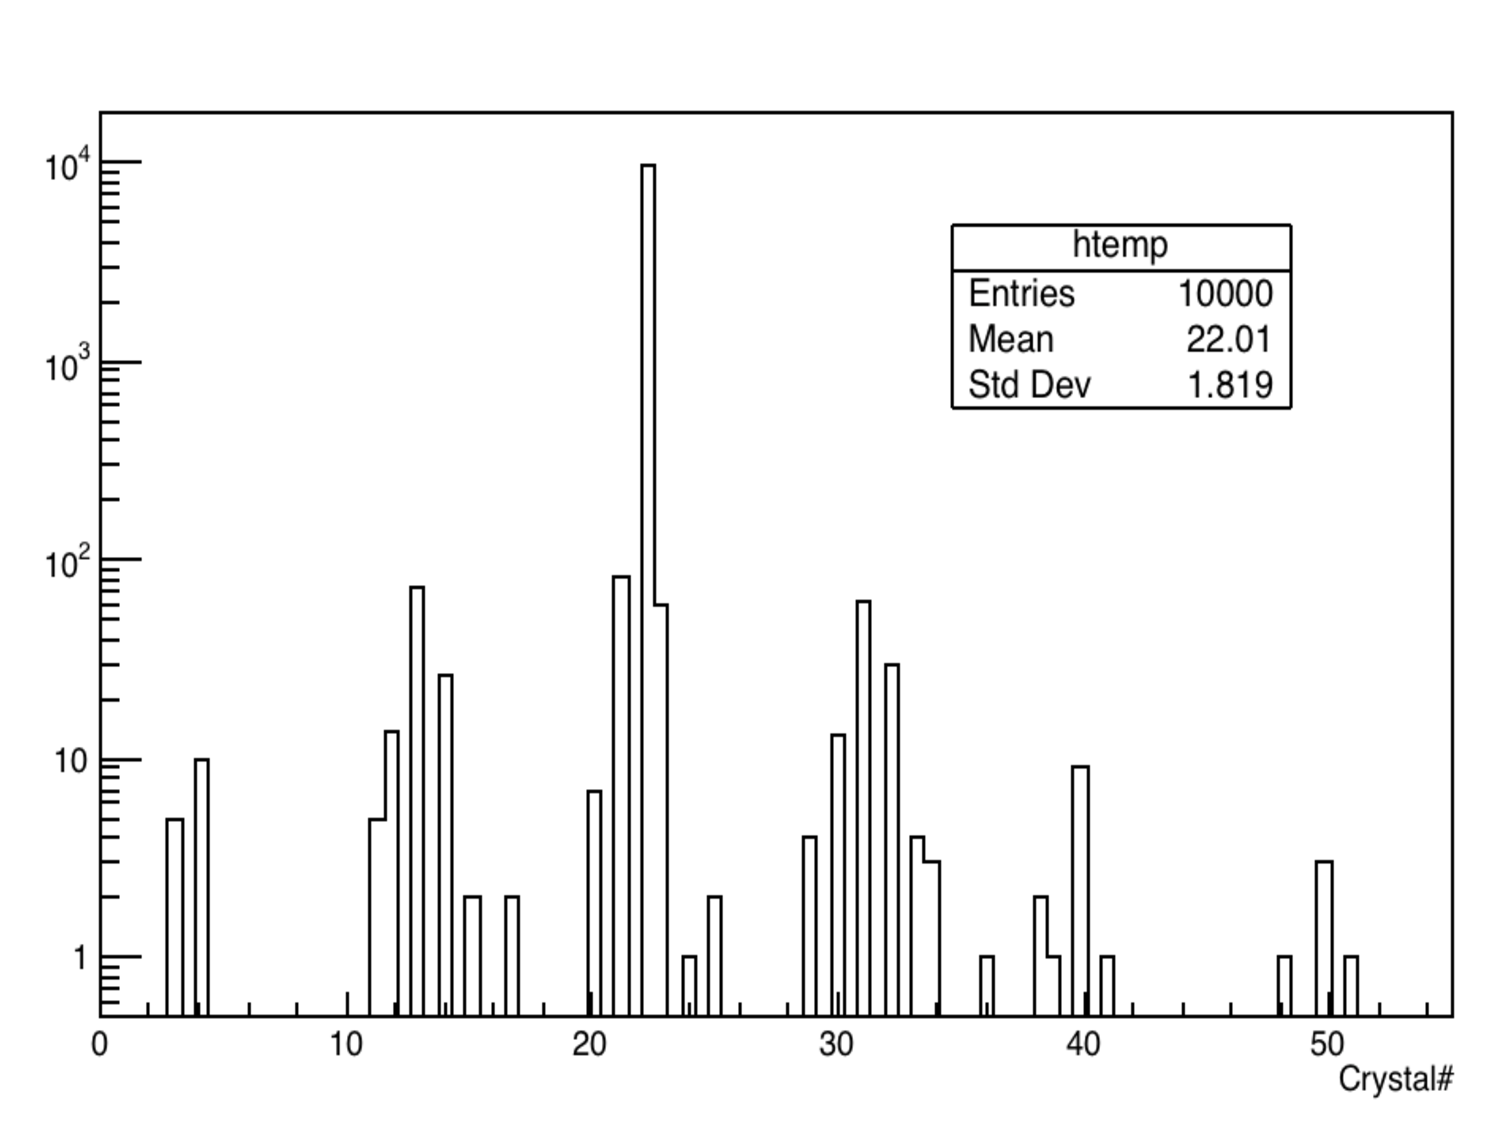
\includegraphics[width=5 cm]{dist_all_center.pdf}
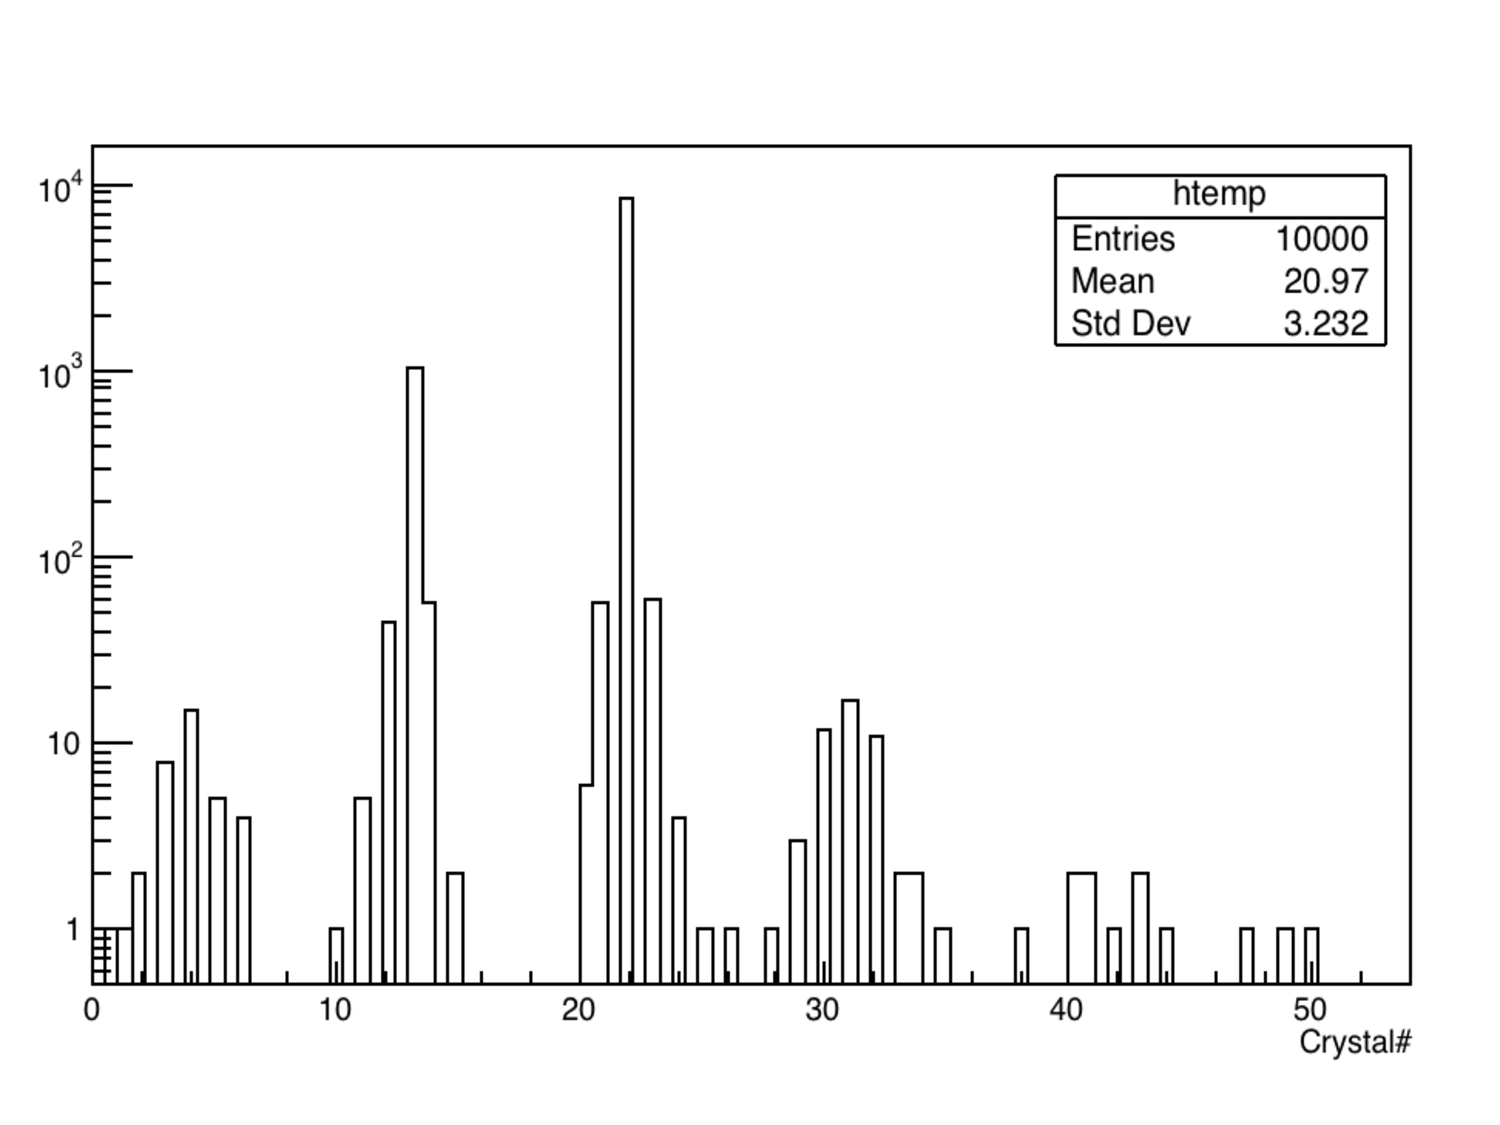
\includegraphics[width=5 cm]{dist_all_bottom.pdf}
%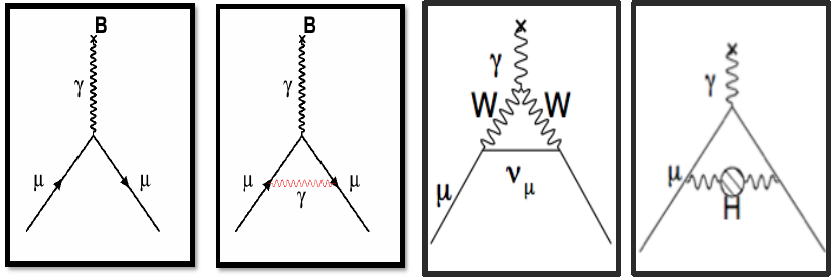
\includegraphics{a_mu_corrections.pdf}
\caption{\label{fig4} The positron  distribution (in log scale) through a 9$\times$6 $\mathrm{PbF_2}$ segmented 
crystals of a calorimeter with exact same conditions as \ref{fig3}.}
\end{figure} 

%%%%%%%%%%%%%%%%%%%%%%%%%%%%%%%%%%%%%%%%%%
\section{Energy spectrum of each crystal}
\begin{figure}[H]
\centering
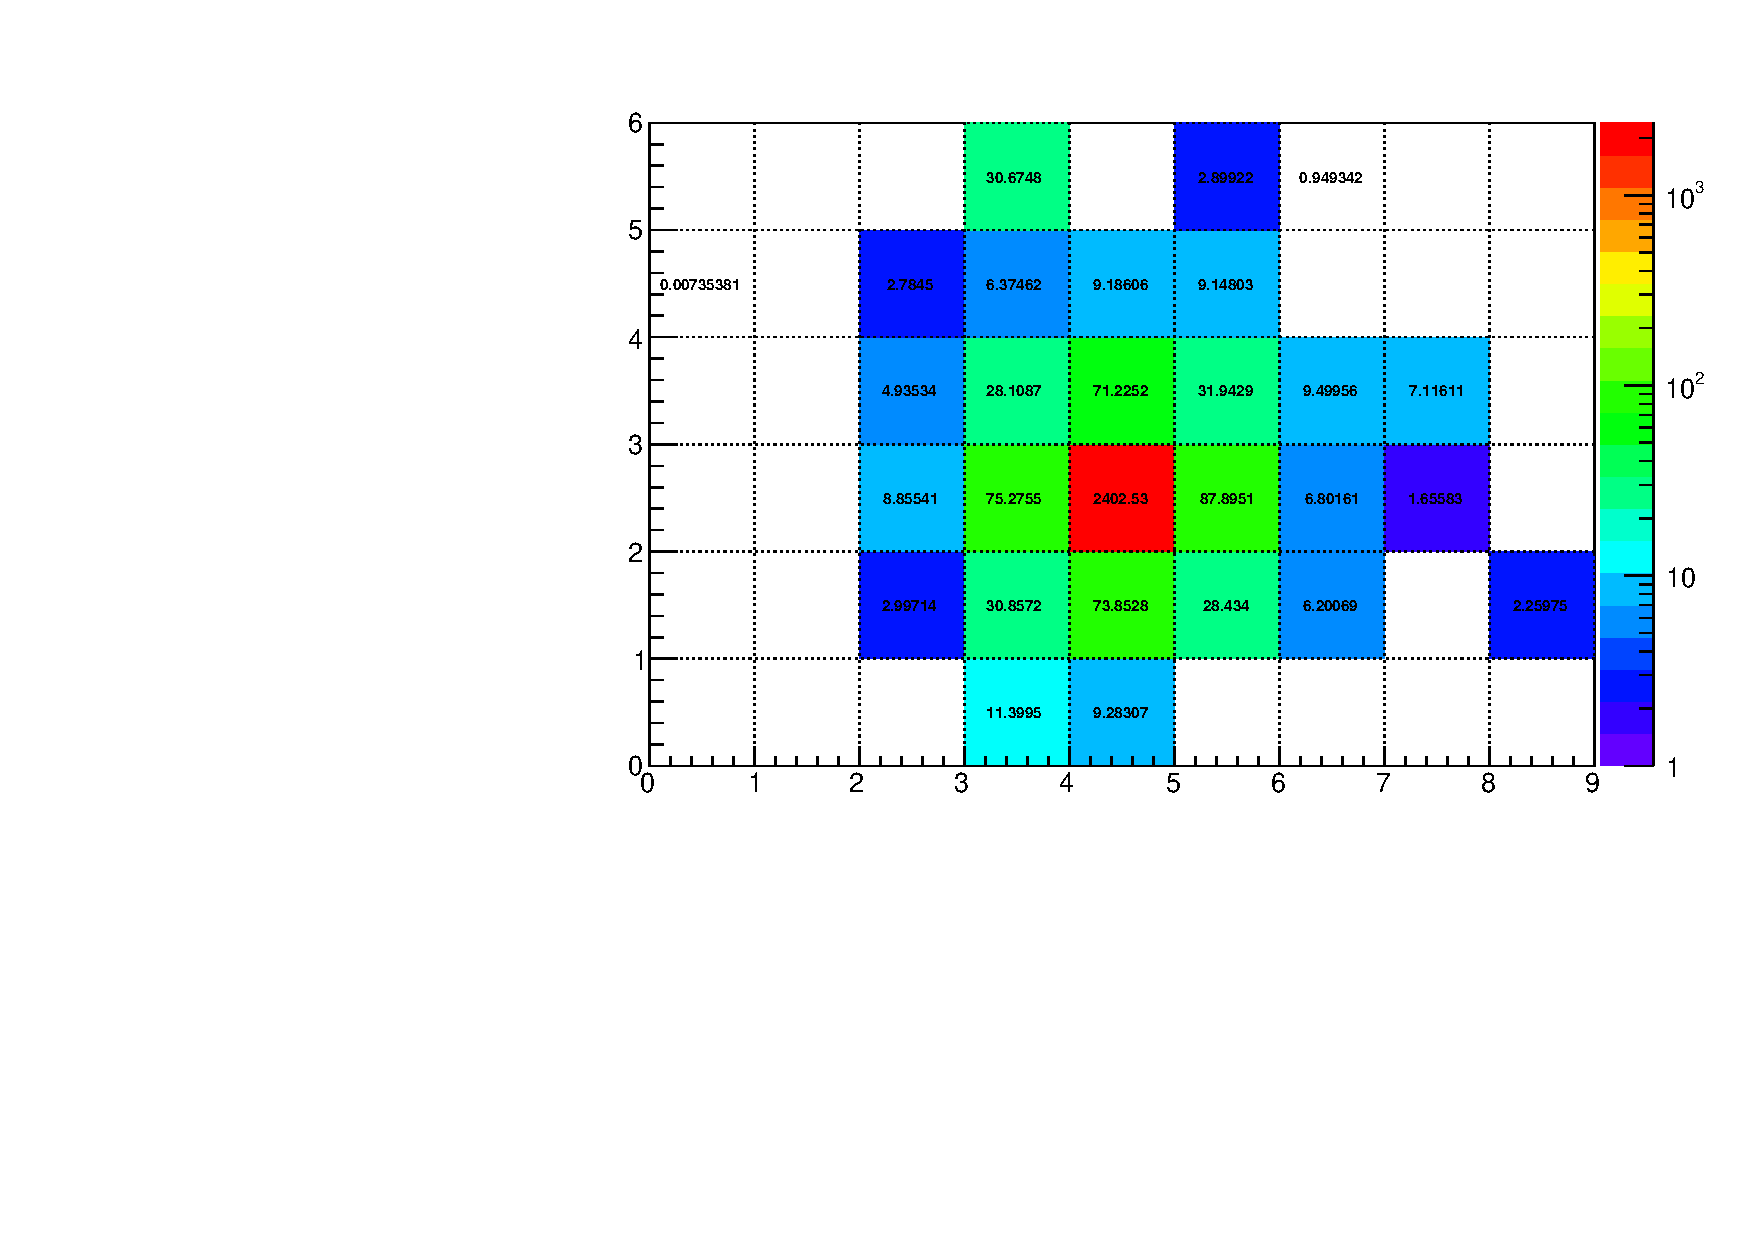
\includegraphics[width=7.5 cm]{energy_crystal_2d.pdf}
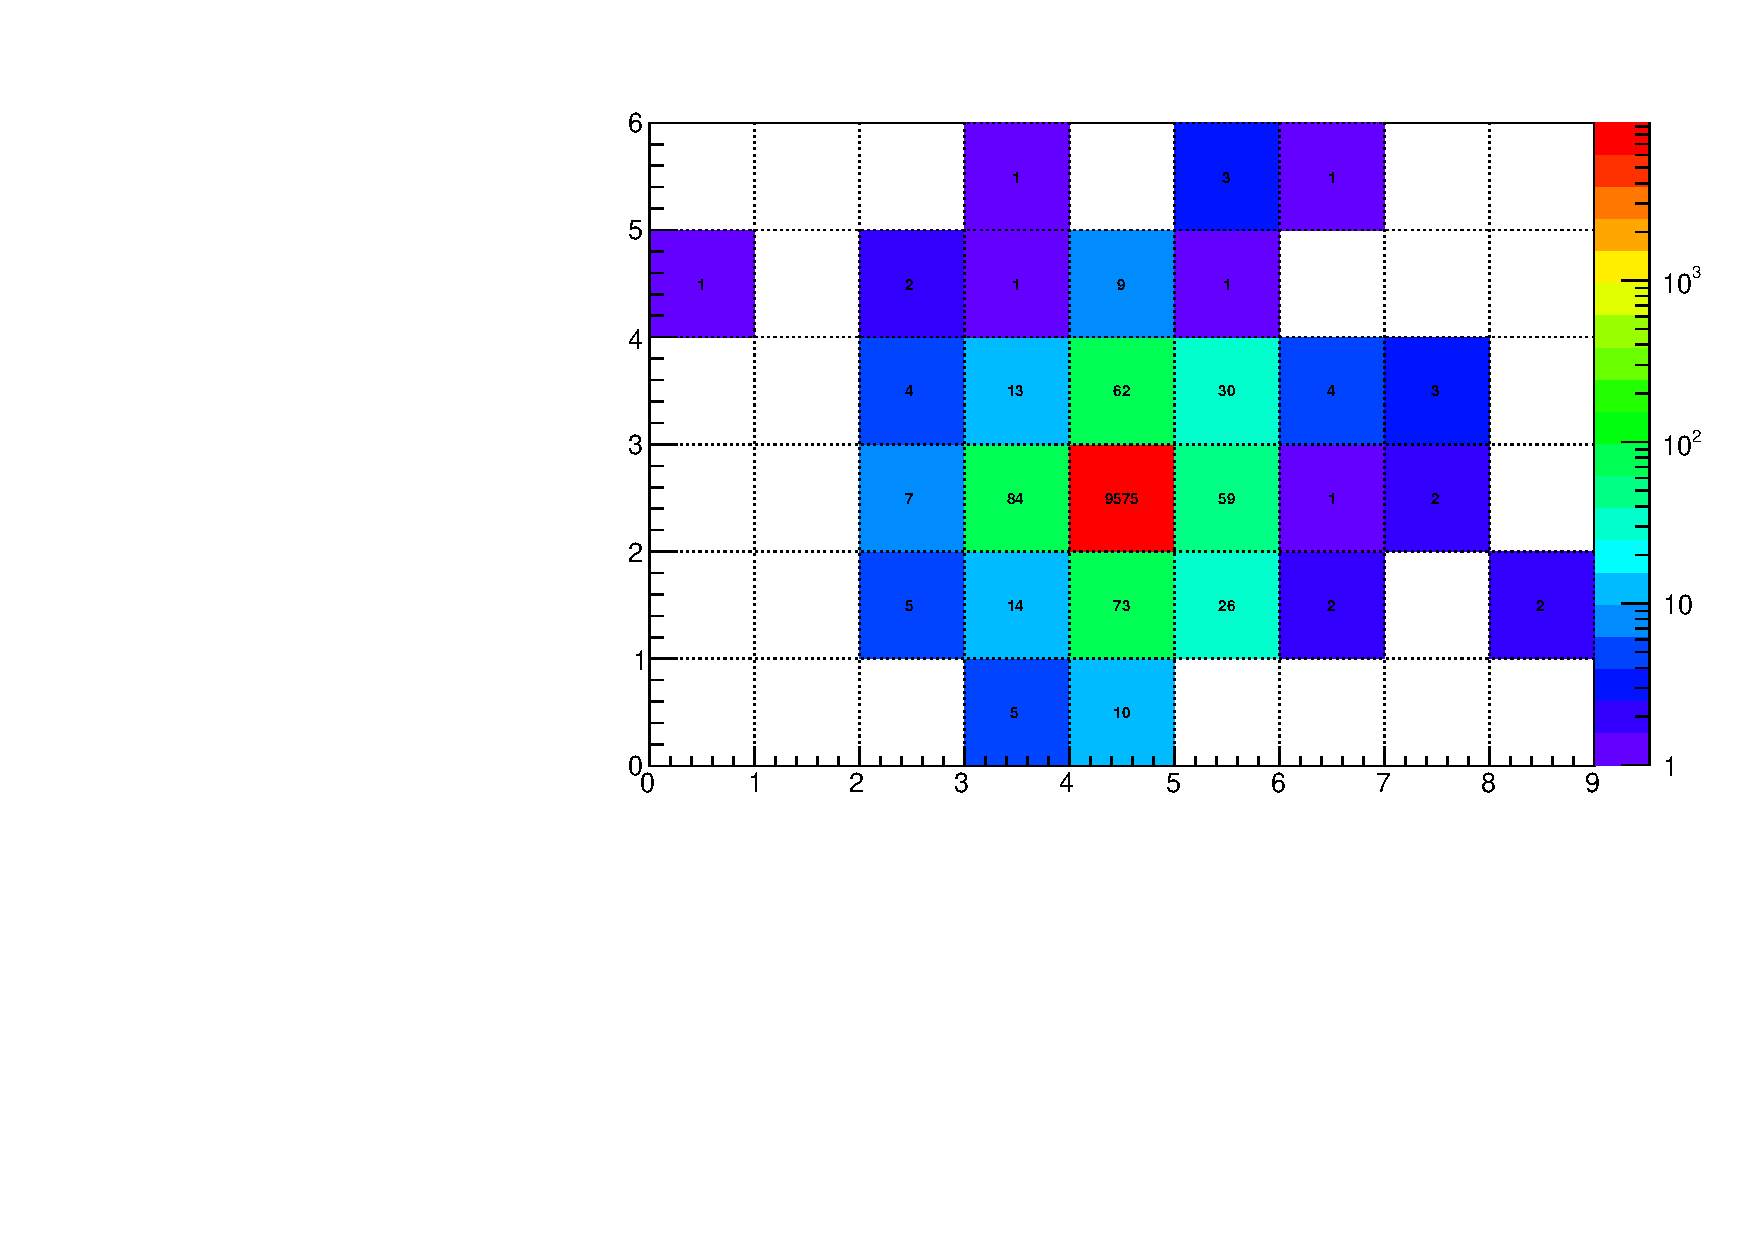
\includegraphics[width=7.5 cm]{no_crystal_2d.pdf}
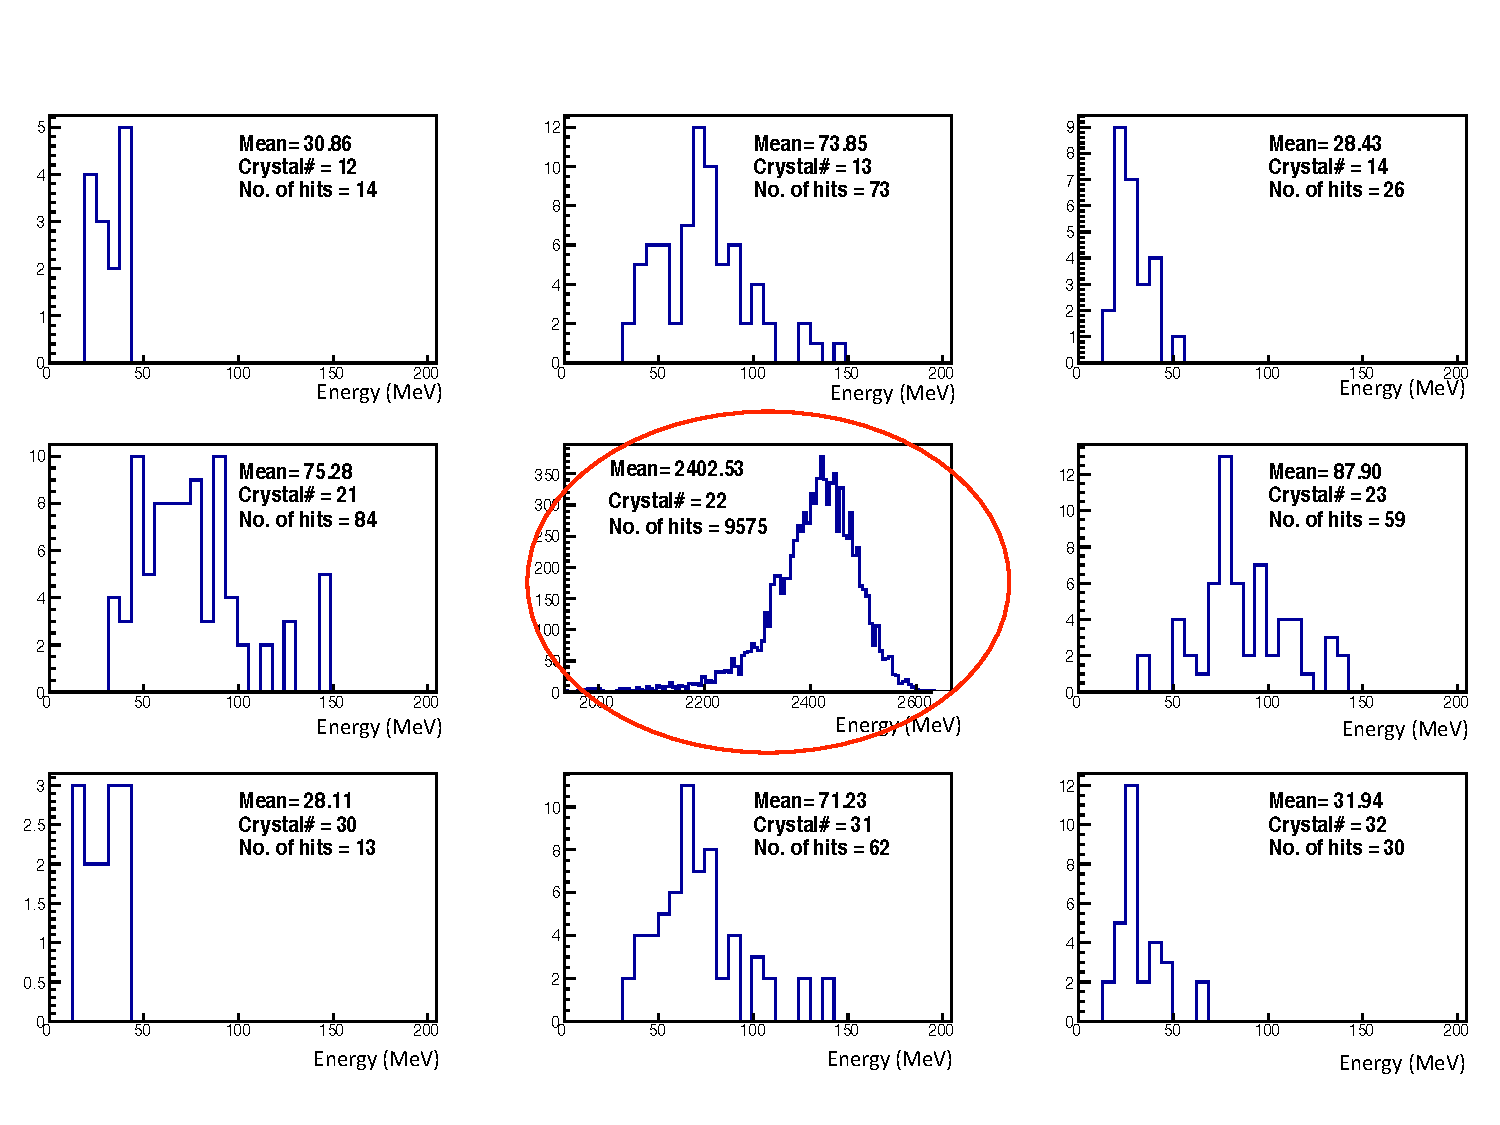
\includegraphics[width=15 cm]{crystal_energy.pdf}
%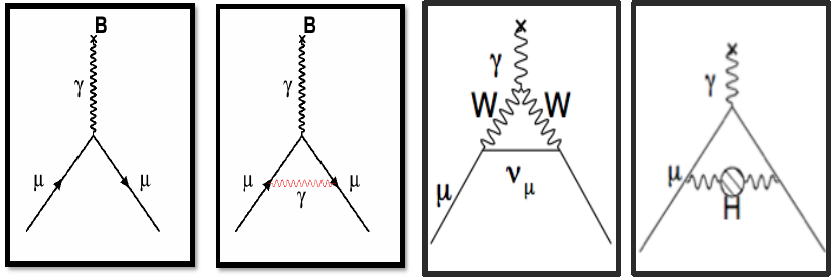
\includegraphics{a_mu_corrections.pdf}
\caption{\label{fig5} Top left: Distribution of mean positron energy for each crystal when the positron 
beam is incident on the center of crystal 22. Top right: Same for occupancy of each crystal.
Bottom: Crystals around the crystal hit (22) showing the actual total energy distribution in these crystals.}
\end{figure}  
\noindent 
A study of the energy distribution on each crystal for 3.1 GeV positron beam incident normally 
on crystal 22 is done in this section. It is obvious that the maximum 
energy will be deposited in crystal 22 and then decrease 
as we move away from this crystal. This is clearly seen in figure \ref{fig5}. 
The left panel of this figure shows the 
energy distribution of each crystal. The number on the crystals here is the mean energy deposited on the crystal. 
The percentage of energy deposited in the central crystal 22 i.e. 2402.53 MeV 
compared to the total energy is 3100 MeV is 77.5\% which matches the value 77.46\% 
of the simulations of TRD (figure 17.3 left). The same holds true for all crystals in the calorimeter. 
The right panel in this figure shows the same for number distribution in each crystal.

The lower panel shows the detailed energy spectrum of each crystal i.e. crystal 22 and the crystals surrounding it. 
The rest of the crystals with really low counts are ignored. 
Note, the fraction of energy deposited in the individual crystals shown in the top left of figure \ref{fig5} matches the values 
of the simulations of TDR (figure 17.3 left) \cite{c3}. 


\section{Variation of incident energy of positron.}

%%%%%%%%%%%%%%%%%%%%%%%%%%%%%%%%%%%%%%%%%%
 
%%%%%%%%%%%%%%%%%%%%%%%%%%%%%%%%%%%%%%%%%%
The total energy of all particles of incident energy of 3.1 GeV is shown in figure \ref{fig2}. 
We varied this energy from 400 MeV to 3100 MeV (in steps of 200 MeV) and investigated the effect. 
The fraction of the mean energy i.e. 2913 MeV wrt the incident energy of 3.1 GeV positrons is 0.9396 
or 93.96\%. This fraction in \% is plotted for incident energies started from 400 MeV 
is shown in the left plot figure \ref{fig6}. 
\begin{figure}[H]
\centering
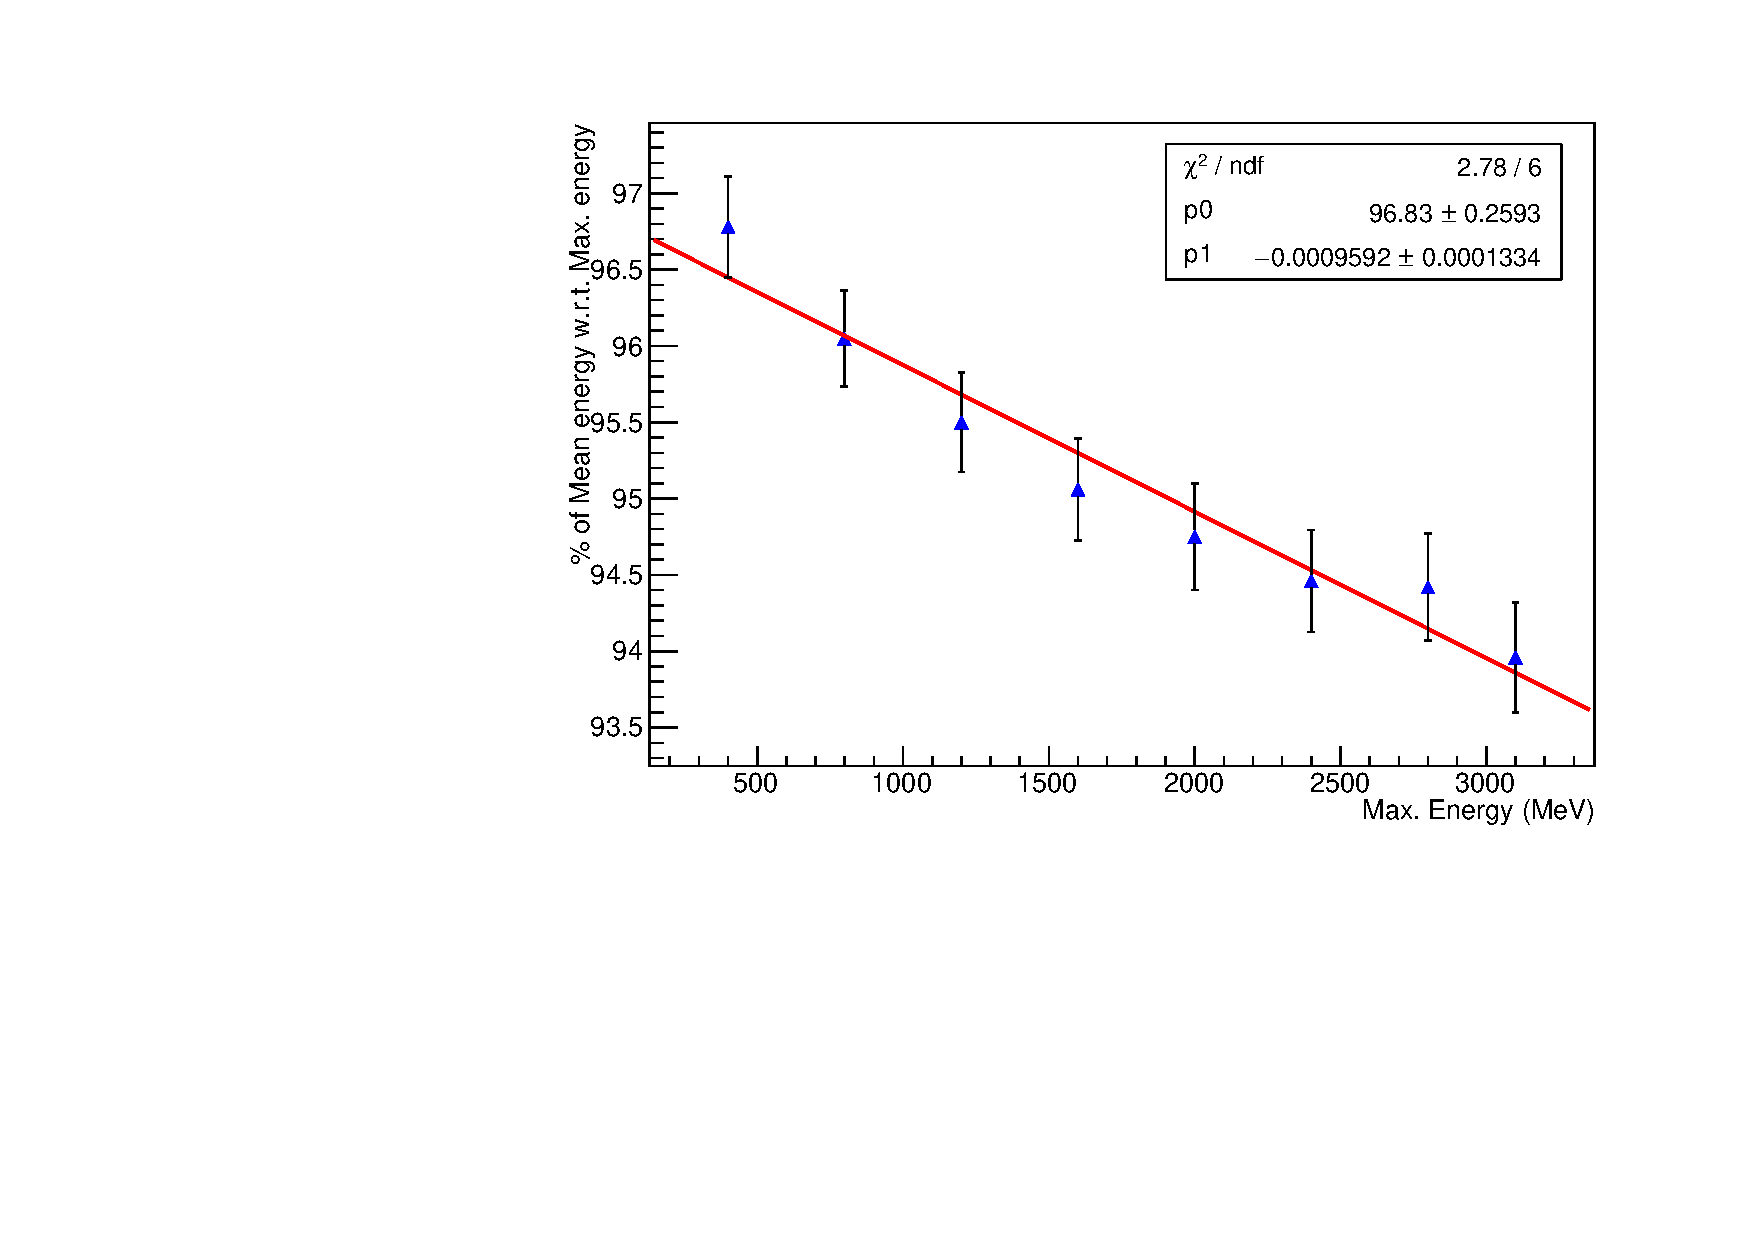
\includegraphics[width=7.5 cm]{mean_fraction.pdf}
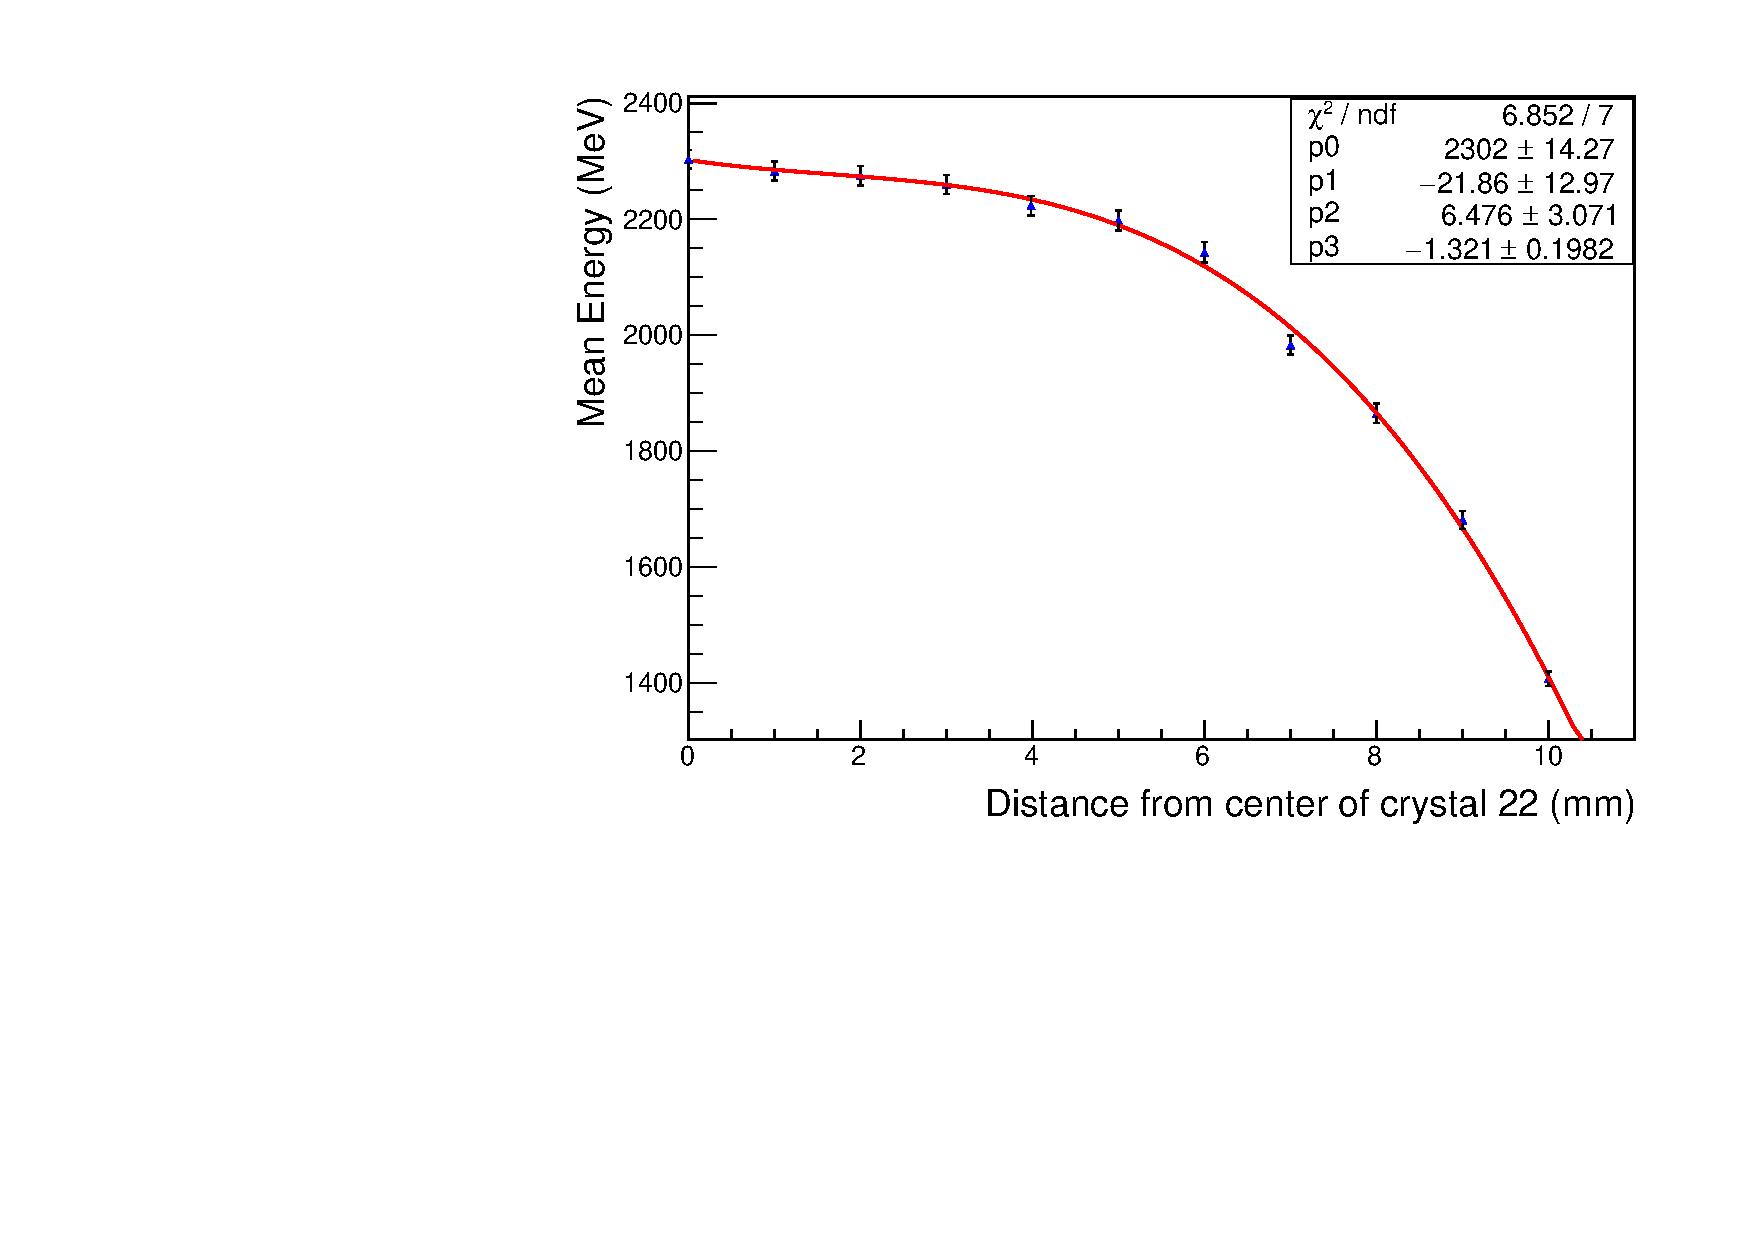
\includegraphics[width=7.5 cm]{mean_tot_energy.pdf}
\caption{\label{fig6}Left: A plot of \% of mean energy compared to the total energy of positrons 
with the total energy varying in steps of 400 MeV, through the 9$\times$6 segmented PbF2 crystals of 
a calorimeter (depicts leakage of positron shower). Right: Plot of mean energy of the positron as a function of beam position.}
\end{figure}
The right plot in figure \ref{fig6} shows the mean energy of all the particles as a function beam position. This plot again was 
done using a simulation with GEANT4. These results match the simulation for the shower leakage into the neighbouring crystals 
as a function of beam position shown in the TDR (figure 17.3 right)\cite{c3}. 
%%%%%%%%%%%%%%%%%%%%%%%%%%%%%%%%%%%%%%%%%%
%=====================================
% References, variant A: internal bibliography
%=====================================
\reftitle{References}
\begin{thebibliography}{999}
% Reference 1
\bibitem{c1}
A.T. Fienberg {\em Measuring the Precession Frequency in the E989 Muon g -- 2 Experiment}. 
PhD thesis, University of Washington, Seatle, 2019.
\bibitem{c2}
A.A. Savchenko et al.{\em ~Geant4 simulations of the lead fluoride calorimeter. Nucl.Instrum.Meth. B402 (2017) 256-262}
\bibitem{c3}
J. Grange et al. {\em Muon (g-2) Technical Design Report, 2015.}
%\bibitem{docdb16402}
%M. Sorbara et al. {\em E989 Note 168: Lost Muon correction for $\omega_a$-europa analysis.}
\end{thebibliography}
\end{document}
